\documentclass[12pt]{article}

%packages
%\usepackage{latexsym}
\usepackage{graphicx}
\usepackage{wrapfig}
\usepackage{color}
\usepackage{amsmath}
\usepackage{dsfont}
\usepackage{placeins}
\usepackage{amssymb}
\usepackage{skull}
\usepackage{enumerate}
\usepackage{soul}
\usepackage{alphalph}
\usepackage{hyperref}
\usepackage{enumerate}
\usepackage{listings}
%\usepackage{fancyhdr}

%\fancyhf{} % clear all header and footers
%\renewcommand{\headrulewidth}{0pt} % remove the header rule
%\fancyfoot[LE, LO]{\thepage}


%\usepackage{pstricks,pst-node,pst-tree}

%\usepackage{algpseudocode}
%\usepackage{amsthm}
%\usepackage{hyperref}
%\usepackage{mathrsfs}
%\usepackage{amsfonts}
%\usepackage{bbding}
%\usepackage{listings}
%\usepackage{appendix}
\usepackage[margin=1in]{geometry}
%\geometry{papersize={8.5in,11in},total={6.5in,9in}}
%\usepackage{cancel}
%\usepackage{algorithmic, algorithm}

\definecolor{dkgreen}{rgb}{0,0.6,0}
\definecolor{gray}{rgb}{0.5,0.5,0.5}
\definecolor{mauve}{rgb}{0.58,0,0.82}
\lstset{ %
  language=R,                     % the language of the code
  basicstyle=\footnotesize,       % the size of the fonts that are used for the code
  numbers=left,                   % where to put the line-numbers
  numberstyle=\tiny\color{gray},  % the style that is used for the line-numbers
  stepnumber=1,                   % the step between two line-numbers. If it's 1, each line
                                  % will be numbered
  numbersep=5pt,                  % how far the line-numbers are from the code
  backgroundcolor=\color{white},  % choose the background color. You must add \usepackage{color}
  showspaces=false,               % show spaces adding particular underscores
  showstringspaces=false,         % underline spaces within strings
  showtabs=false,                 % show tabs within strings adding particular underscores
  frame=single,                   % adds a frame around the code
  rulecolor=\color{black},        % if not set, the frame-color may be changed on line-breaks within not-black text (e.g. commens (green here))
  tabsize=2,                      % sets default tabsize to 2 spaces
  captionpos=b,                   % sets the caption-position to bottom
  breaklines=true,                % sets automatic line breaking
  breakatwhitespace=false,        % sets if automatic breaks should only happen at whitespace
  title=\lstname,                 % show the filename of files included with \lstinputlisting;
                                  % also try caption instead of title
  keywordstyle=\color{blue},      % keyword style
  commentstyle=\color{dkgreen},   % comment style
  stringstyle=\color{mauve},      % string literal style
  escapeinside={\%*}{*)},         % if you want to add a comment within your code
  morekeywords={*,...}            % if you want to add more keywords to the set
}

\newcommand{\qu}[1]{``#1''}
\newcommand{\spc}[1]{\\ \vspace{#1cm}}

\newcounter{probnum}
\setcounter{probnum}{1}
\newcounter{numpts}
\setcounter{numpts}{0}

%create definition to allow local margin changes
\def\changemargin#1#2{\list{}{\rightmargin#2\leftmargin#1}\item[]}
\let\endchangemargin=\endlist 

%allow equations to span multiple pages
\allowdisplaybreaks

%define colors and color typesetting conveniences
\definecolor{gray}{rgb}{0.5,0.5,0.5}
\definecolor{black}{rgb}{0,0,0}
\definecolor{white}{rgb}{1,1,1}
\definecolor{blue}{rgb}{0.5,0.5,1}
\newcommand{\inblue}[1]{\color{blue}#1 \color{black}}
\definecolor{green}{rgb}{0.133,0.545,0.133}
\newcommand{\ingreen}[1]{\color{green}#1 \color{black}}
\definecolor{yellow}{rgb}{1,0.549,0}
\newcommand{\inyellow}[1]{\color{yellow}#1 \color{black}}
\definecolor{red}{rgb}{1,0.133,0.133}
\newcommand{\inred}[1]{\color{red}#1 \color{black}}
\definecolor{purple}{rgb}{0.58,0,0.827}
\newcommand{\inpurple}[1]{\color{purple}#1 \color{black}}
\definecolor{gray}{rgb}{0.5,0.5,0.5}
\newcommand{\ingray}[1]{\color{gray}#1 \color{black}}
\definecolor{backgcode}{rgb}{0.97,0.97,0.8}
\definecolor{Brown}{cmyk}{0,0.81,1,0.60}
\definecolor{OliveGreen}{cmyk}{0.64,0,0.95,0.40}
\definecolor{CadetBlue}{cmyk}{0.62,0.57,0.23,0}

%define new math operators
\DeclareMathOperator*{\argmax}{arg\,max~}
\DeclareMathOperator*{\argmin}{arg\,min~}
\DeclareMathOperator*{\argsup}{arg\,sup~}
\DeclareMathOperator*{\arginf}{arg\,inf~}
\DeclareMathOperator*{\convolution}{\text{\Huge{$\ast$}}}
\newcommand{\infconv}[2]{\convolution^\infty_{#1 = 1} #2}
%true functions

%%%% GENERAL SHORTCUTS

\makeatletter
\newalphalph{\alphmult}[mult]{\@alph}{26}
\renewcommand{\labelenumi}{(\alphmult{\value{enumi}})}
\renewcommand{\theenumi}{\AlphAlph{\value{enumi}}}
\makeatother
%shortcuts for pure typesetting conveniences
\newcommand{\bv}[1]{\boldsymbol{#1}}

%shortcuts for compound constants
\newcommand{\BetaDistrConst}{\dfrac{\Gamma(\alpha + \beta)}{\Gamma(\alpha)\Gamma(\beta)}}
\newcommand{\NormDistrConst}{\dfrac{1}{\sqrt{2\pi\sigma^2}}}

%shortcuts for conventional symbols
\newcommand{\tsq}{\tau^2}
\newcommand{\tsqh}{\hat{\tau}^2}
\newcommand{\sigsq}{\sigma^2}
\newcommand{\sigsqsq}{\parens{\sigma^2}^2}
\newcommand{\sigsqovern}{\dfrac{\sigsq}{n}}
\newcommand{\tausq}{\tau^2}
\newcommand{\tausqalpha}{\tau^2_\alpha}
\newcommand{\tausqbeta}{\tau^2_\beta}
\newcommand{\tausqsigma}{\tau^2_\sigma}
\newcommand{\betasq}{\beta^2}
\newcommand{\sigsqvec}{\bv{\sigma}^2}
\newcommand{\sigsqhat}{\hat{\sigma}^2}
\newcommand{\sigsqhatmlebayes}{\sigsqhat_{\text{Bayes, MLE}}}
\newcommand{\sigsqhatmle}[1]{\sigsqhat_{#1, \text{MLE}}}
\newcommand{\bSigma}{\bv{\Sigma}}
\newcommand{\bSigmainv}{\bSigma^{-1}}
\newcommand{\thetavec}{\bv{\theta}}
\newcommand{\thetahat}{\hat{\theta}}
\newcommand{\thetahatmle}{\hat{\theta}_{\mathrm{MLE}}}
\newcommand{\thetavechatmle}{\hat{\thetavec}_{\mathrm{MLE}}}
\newcommand{\muhat}{\hat{\mu}}
\newcommand{\musq}{\mu^2}
\newcommand{\muvec}{\bv{\mu}}
\newcommand{\muhatmle}{\muhat_{\text{MLE}}}
\newcommand{\lambdahat}{\hat{\lambda}}
\newcommand{\lambdahatmle}{\lambdahat_{\text{MLE}}}
\newcommand{\thetahatmap}{\hat{\theta}_{\mathrm{MAP}}}
\newcommand{\thetahatmae}{\hat{\theta}_{\mathrm{MAE}}}
\newcommand{\thetahatmmse}{\hat{\theta}_{\mathrm{MMSE}}}
\newcommand{\etavec}{\bv{\eta}}
\newcommand{\alphavec}{\bv{\alpha}}
\newcommand{\minimaxdec}{\delta^*_{\mathrm{mm}}}
\newcommand{\ybar}{\bar{y}}
\newcommand{\xbar}{\bar{x}}
\newcommand{\Xbar}{\bar{X}}
\newcommand{\iid}{~{\buildrel iid \over \sim}~}
\newcommand{\inddist}{~{\buildrel ind \over \sim}~}
\newcommand{\approxdist}{~{\buildrel approx \over \sim}~}
\newcommand{\equalsindist}{~{\buildrel d \over =}~}
\newcommand{\loglik}[1]{\ell\parens{#1}}
\newcommand{\thetahatkminone}{\thetahat^{(k-1)}}
\newcommand{\thetahatkplusone}{\thetahat^{(k+1)}}
\newcommand{\thetahatk}{\thetahat^{(k)}}
\newcommand{\half}{\frac{1}{2}}
\newcommand{\third}{\frac{1}{3}}
\newcommand{\twothirds}{\frac{2}{3}}
\newcommand{\fourth}{\frac{1}{4}}
\newcommand{\fifth}{\frac{1}{5}}
\newcommand{\sixth}{\frac{1}{6}}

%shortcuts for vector and matrix notation
\newcommand{\A}{\bv{A}}
\newcommand{\At}{\A^T}
\renewcommand{\H}{\bv{H}}
\newcommand{\Ht}{\H^\top}
\newcommand{\Ainv}{\inverse{\A}}
\newcommand{\B}{\bv{B}}
\newcommand{\K}{\bv{K}}
\newcommand{\Kt}{\K^T}
\newcommand{\Kinv}{\inverse{K}}
\newcommand{\Kinvt}{(\Kinv)^T}
\newcommand{\M}{\bv{M}}
\newcommand{\Bt}{\B^T}
\newcommand{\Q}{\bv{Q}}
\newcommand{\Qt}{\Q^T}
\newcommand{\R}{\bv{R}}
\newcommand{\Rt}{\R^T}
\newcommand{\Z}{\bv{Z}}
\newcommand{\X}{\bv{X}}
\renewcommand{\b}{\bv{b}}
\newcommand{\Xsub}{\X_{\text{(sub)}}}
\newcommand{\Xsubadj}{\X_{\text{(sub,adj)}}}
\newcommand{\I}{\bv{I}}
\newcommand{\Y}{\bv{Y}}
\newcommand{\sigsqI}{\sigsq\I}
\renewcommand{\P}{\bv{P}}
\newcommand{\Psub}{\P_{\text{(sub)}}}
\newcommand{\Pt}{\P^T}
\newcommand{\Pii}{P_{ii}}
\newcommand{\Pij}{P_{ij}}
\newcommand{\IminP}{(\I-\P)}
\newcommand{\Xt}{\bv{X}^T}
\newcommand{\XtX}{\Xt\X}
\newcommand{\XtXinv}{\parens{\Xt\X}^{-1}}
\newcommand{\XtXinvXt}{\XtXinv\Xt}
\newcommand{\XXtXinvXt}{\X\XtXinvXt}
\newcommand{\x}{\bv{x}}
\newcommand{\w}{\bv{w}}
\newcommand{\onevec}{\bv{1}}
\newcommand{\oneton}{1, \ldots, n}
\newcommand{\yoneton}{y_1, \ldots, y_n}
\newcommand{\yonetonorder}{y_{(1)}, \ldots, y_{(n)}}
\newcommand{\Yoneton}{Y_1, \ldots, Y_n}
\newcommand{\iinoneton}{i \in \braces{\oneton}}
\newcommand{\onetom}{1, \ldots, m}
\newcommand{\jinonetom}{j \in \braces{\onetom}}
\newcommand{\xoneton}{x_1, \ldots, x_n}
\newcommand{\Xoneton}{X_1, \ldots, X_n}
\newcommand{\xt}{\x^T}
\newcommand{\y}{\bv{y}}
\newcommand{\yt}{\y^T}
\renewcommand{\c}{\bv{c}}
\newcommand{\ct}{\c^T}
\newcommand{\tstar}{\bv{t}^*}
\renewcommand{\u}{\bv{u}}
\renewcommand{\v}{\bv{v}}
\renewcommand{\a}{\bv{a}}
\newcommand{\s}{\bv{s}}
\newcommand{\yadj}{\y_{\text{(adj)}}}
\newcommand{\xjadj}{\x_{j\text{(adj)}}}
\newcommand{\xjadjM}{\x_{j \perp M}}
\newcommand{\yhat}{\hat{\y}}
\newcommand{\yhatsub}{\yhat_{\text{(sub)}}}
\newcommand{\yhatstar}{\yhat^*}
\newcommand{\yhatstarnew}{\yhatstar_{\text{new}}}
\newcommand{\z}{\bv{z}}
\newcommand{\zt}{\z^T}
\newcommand{\bb}{\bv{b}}
\newcommand{\bbt}{\bb^T}
\newcommand{\bbeta}{\bv{\beta}}
\newcommand{\beps}{\bv{\epsilon}}
\newcommand{\bepst}{\beps^T}
\newcommand{\e}{\bv{e}}
\newcommand{\Mofy}{\M(\y)}
\newcommand{\KofAlpha}{K(\alpha)}
\newcommand{\ellset}{\mathcal{L}}
\newcommand{\oneminalph}{1-\alpha}
\newcommand{\SSE}{\text{SSE}}
\newcommand{\SSEsub}{\text{SSE}_{\text{(sub)}}}
\newcommand{\MSE}{\text{MSE}}
\newcommand{\RMSE}{\text{RMSE}}
\newcommand{\SSR}{\text{SSR}}
\newcommand{\SST}{\text{SST}}
\newcommand{\JSest}{\delta_{\text{JS}}(\x)}
\newcommand{\Bayesest}{\delta_{\text{Bayes}}(\x)}
\newcommand{\EmpBayesest}{\delta_{\text{EmpBayes}}(\x)}
\newcommand{\BLUPest}{\delta_{\text{BLUP}}}
\newcommand{\MLEest}[1]{\hat{#1}_{\text{MLE}}}

%shortcuts for Linear Algebra stuff (i.e. vectors and matrices)
\newcommand{\twovec}[2]{\bracks{\begin{array}{c} #1 \\ #2 \end{array}}}
\newcommand{\threevec}[3]{\bracks{\begin{array}{c} #1 \\ #2 \\ #3 \end{array}}}
\newcommand{\fivevec}[5]{\bracks{\begin{array}{c} #1 \\ #2 \\ #3 \\ #4 \\ #5 \end{array}}}
\newcommand{\twobytwomat}[4]{\bracks{\begin{array}{cc} #1 & #2 \\ #3 & #4 \end{array}}}
\newcommand{\threebytwomat}[6]{\bracks{\begin{array}{cc} #1 & #2 \\ #3 & #4 \\ #5 & #6 \end{array}}}

%shortcuts for conventional compound symbols
\newcommand{\thetainthetas}{\theta \in \Theta}
\newcommand{\reals}{\mathbb{R}}
\newcommand{\complexes}{\mathbb{C}}
\newcommand{\rationals}{\mathbb{Q}}
\newcommand{\integers}{\mathbb{Z}}
\newcommand{\naturals}{\mathbb{N}}
\newcommand{\forallninN}{~~\forall n \in \naturals}
\newcommand{\forallxinN}[1]{~~\forall #1 \in \reals}
\newcommand{\matrixdims}[2]{\in \reals^{\,#1 \times #2}}
\newcommand{\inRn}[1]{\in \reals^{\,#1}}
\newcommand{\mathimplies}{\quad\Rightarrow\quad}
\newcommand{\mathlogicequiv}{\quad\Leftrightarrow\quad}
\newcommand{\eqncomment}[1]{\quad \text{(#1)}}
\newcommand{\limitn}{\lim_{n \rightarrow \infty}}
\newcommand{\limitN}{\lim_{N \rightarrow \infty}}
\newcommand{\limitd}{\lim_{d \rightarrow \infty}}
\newcommand{\limitt}{\lim_{t \rightarrow \infty}}
\newcommand{\limitsupn}{\limsup_{n \rightarrow \infty}~}
\newcommand{\limitinfn}{\liminf_{n \rightarrow \infty}~}
\newcommand{\limitk}{\lim_{k \rightarrow \infty}}
\newcommand{\limsupn}{\limsup_{n \rightarrow \infty}}
\newcommand{\limsupk}{\limsup_{k \rightarrow \infty}}
\newcommand{\floor}[1]{\left\lfloor #1 \right\rfloor}
\newcommand{\ceil}[1]{\left\lceil #1 \right\rceil}

%shortcuts for environments
\newcommand{\beqn}{\vspace{-0.25cm}\begin{eqnarray*}}
\newcommand{\eeqn}{\end{eqnarray*}}
\newcommand{\bneqn}{\vspace{-0.25cm}\begin{eqnarray}}
\newcommand{\eneqn}{\end{eqnarray}}
\newcommand{\benum}{\begin{enumerate}}
\newcommand{\eenum}{\end{enumerate}}

%shortcuts for mini environments
\newcommand{\parens}[1]{\left(#1\right)}
\newcommand{\squared}[1]{\parens{#1}^2}
\newcommand{\tothepow}[2]{\parens{#1}^{#2}}
\newcommand{\prob}[1]{\mathbb{P}\parens{#1}}
\newcommand{\littleo}[1]{o\parens{#1}}
\newcommand{\bigo}[1]{O\parens{#1}}
\newcommand{\Lp}[1]{\mathbb{L}^{#1}}
\renewcommand{\arcsin}[1]{\text{arcsin}\parens{#1}}
\newcommand{\prodonen}[2]{\bracks{\prod_{#1=1}^n #2}}
\newcommand{\mysum}[4]{\sum_{#1=#2}^{#3} #4}
\newcommand{\sumonen}[2]{\sum_{#1=1}^n #2}
\newcommand{\infsum}[2]{\sum_{#1=1}^\infty #2}
\newcommand{\infprod}[2]{\prod_{#1=1}^\infty #2}
\newcommand{\infunion}[2]{\bigcup_{#1=1}^\infty #2}
\newcommand{\infinter}[2]{\bigcap_{#1=1}^\infty #2}
\newcommand{\infintegral}[2]{\int^\infty_{-\infty} #2 ~\text{d}#1}
\newcommand{\supthetas}[1]{\sup_{\thetainthetas}\braces{#1}}
\newcommand{\bracks}[1]{\left[#1\right]}
\newcommand{\braces}[1]{\left\{#1\right\}}
\newcommand{\set}[1]{\left\{#1\right\}}
\newcommand{\abss}[1]{\left|#1\right|}
\newcommand{\norm}[1]{\left|\left|#1\right|\right|}
\newcommand{\normsq}[1]{\norm{#1}^2}
\newcommand{\inverse}[1]{\parens{#1}^{-1}}
\newcommand{\rowof}[2]{\parens{#1}_{#2\cdot}}

%shortcuts for functionals
\newcommand{\realcomp}[1]{\text{Re}\bracks{#1}}
\newcommand{\imagcomp}[1]{\text{Im}\bracks{#1}}
\newcommand{\range}[1]{\text{range}\bracks{#1}}
\newcommand{\colsp}[1]{\text{colsp}\bracks{#1}}
\newcommand{\rowsp}[1]{\text{rowsp}\bracks{#1}}
\newcommand{\tr}[1]{\text{tr}\bracks{#1}}
\newcommand{\rank}[1]{\text{rank}\bracks{#1}}
\newcommand{\proj}[2]{\text{Proj}_{#1}\bracks{#2}}
\newcommand{\projcolspX}[1]{\text{Proj}_{\colsp{\X}}\bracks{#1}}
\newcommand{\median}[1]{\text{median}\bracks{#1}}
\newcommand{\mean}[1]{\text{mean}\bracks{#1}}
\newcommand{\dime}[1]{\text{dim}\bracks{#1}}
\renewcommand{\det}[1]{\text{det}\bracks{#1}}
\newcommand{\expe}[1]{\mathbb{E}\bracks{#1}}
\newcommand{\expeabs}[1]{\expe{\abss{#1}}}
\newcommand{\expesub}[2]{\mathbb{E}_{#1}\bracks{#2}}
\newcommand{\cexpesub}[3]{\mathbb{E}_{#1}\bracks{#2~|~#3}}
\newcommand{\indic}[1]{\mathds{1}_{#1}}
\newcommand{\var}[1]{\mathbb{V}\text{ar}\bracks{#1}}
\newcommand{\sd}[1]{\mathbb{S}\text{D}\bracks{#1}}
\newcommand{\cov}[2]{\text{Cov}\bracks{#1, #2}}
\newcommand{\corr}[2]{\text{Corr}\bracks{#1, #2}}
\newcommand{\se}[1]{\text{SE}\bracks{#1}}
\newcommand{\seest}[1]{\hat{\text{SE}}\bracks{#1}}
\newcommand{\bias}[1]{\text{Bias}\bracks{#1}}
\newcommand{\partialop}[2]{\dfrac{\partial}{\partial #1}\bracks{#2}}
\newcommand{\secpartialop}[2]{\dfrac{\partial^2}{\partial #1^2}\bracks{#2}}
\newcommand{\mixpartialop}[3]{\dfrac{\partial^2}{\partial #1 \partial #2}\bracks{#3}}

%shortcuts for functions
\renewcommand{\exp}[1]{\mathrm{exp}\parens{#1}}
\renewcommand{\cos}[1]{\text{cos}\parens{#1}}
\renewcommand{\sin}[1]{\text{sin}\parens{#1}}
\newcommand{\sign}[1]{\text{sign}\parens{#1}}
\newcommand{\are}[1]{\mathrm{ARE}\parens{#1}}
\newcommand{\natlog}[1]{\ln\parens{#1}}
\newcommand{\oneover}[1]{\frac{1}{#1}}
\newcommand{\overtwo}[1]{\frac{#1}{2}}
\newcommand{\overn}[1]{\frac{#1}{n}}
\newcommand{\oneoversqrt}[1]{\oneover{\sqrt{#1}}}
\newcommand{\sqd}[1]{\parens{#1}^2}
\newcommand{\loss}[1]{\ell\parens{\theta, #1}}
\newcommand{\losstwo}[2]{\ell\parens{#1, #2}}
\newcommand{\cf}{\phi(t)}

%English language specific shortcuts
\newcommand{\ie}{\textit{i.e.} }
\newcommand{\AKA}{\textit{AKA} }
\renewcommand{\iff}{\textit{iff}}
\newcommand{\eg}{\textit{e.g.} }
\renewcommand{\st}{\textit{s.t.} }
\newcommand{\wrt}{\textit{w.r.t.} }
\newcommand{\mathst}{~~\text{\st}~~}
\newcommand{\mathand}{~~\text{and}~~}
\newcommand{\ala}{\textit{a la} }
\newcommand{\ppp}{posterior predictive p-value}
\newcommand{\dd}{dataset-to-dataset}

%shortcuts for distribution titles
\newcommand{\logistic}[2]{\mathrm{Logistic}\parens{#1,\,#2}}
\newcommand{\bernoulli}[1]{\mathrm{Bernoulli}\parens{#1}}
\newcommand{\betanot}[2]{\mathrm{Beta}\parens{#1,\,#2}}
\newcommand{\stdbetanot}{\betanot{\alpha}{\beta}}
\newcommand{\multnormnot}[3]{\mathcal{N}_{#1}\parens{#2,\,#3}}
\newcommand{\normnot}[2]{\mathcal{N}\parens{#1,\,#2}}
\newcommand{\classicnormnot}{\normnot{\mu}{\sigsq}}
\newcommand{\stdnormnot}{\normnot{0}{1}}
\newcommand{\uniform}[2]{\mathrm{U}\parens{#1,\,#2}}
\newcommand{\stduniform}{\uniform{0}{1}}
\newcommand{\exponential}[1]{\mathrm{Exp}\parens{#1}}
\newcommand{\gammadist}[2]{\mathrm{Gamma}\parens{#1, #2}}
\newcommand{\poisson}[1]{\mathrm{Poisson}\parens{#1}}
\newcommand{\binomial}[2]{\mathrm{Binomial}\parens{#1,\,#2}}
\newcommand{\rayleigh}[1]{\mathrm{Rayleigh}\parens{#1}}
\newcommand{\multinomial}[2]{\mathrm{Multinomial}\parens{#1,\,#2}}
\newcommand{\gammanot}[2]{\mathrm{Gamma}\parens{#1,\,#2}}
\newcommand{\cauchynot}[2]{\text{Cauchy}\parens{#1,\,#2}}
\newcommand{\invchisqnot}[1]{\text{Inv}\chisq{#1}}
\newcommand{\invscaledchisqnot}[2]{\text{ScaledInv}\ncchisq{#1}{#2}}
\newcommand{\invgammanot}[2]{\text{InvGamma}\parens{#1,\,#2}}
\newcommand{\chisq}[1]{\chi^2_{#1}}
\newcommand{\ncchisq}[2]{\chi^2_{#1}\parens{#2}}
\newcommand{\ncF}[3]{F_{#1,#2}\parens{#3}}

%shortcuts for PDF's of common distributions
\newcommand{\logisticpdf}[3]{\oneover{#3}\dfrac{\exp{-\dfrac{#1 - #2}{#3}}}{\parens{1+\exp{-\dfrac{#1 - #2}{#3}}}^2}}
\newcommand{\betapdf}[3]{\dfrac{\Gamma(#2 + #3)}{\Gamma(#2)\Gamma(#3)}#1^{#2-1} (1-#1)^{#3-1}}
\newcommand{\normpdf}[3]{\frac{1}{\sqrt{2\pi#3}}\exp{-\frac{1}{2#3}(#1 - #2)^2}}
\newcommand{\normpdfvarone}[2]{\dfrac{1}{\sqrt{2\pi}}e^{-\half(#1 - #2)^2}}
\newcommand{\chisqpdf}[2]{\dfrac{1}{2^{#2/2}\Gamma(#2/2)}\; {#1}^{#2/2-1} e^{-#1/2}}
\newcommand{\invchisqpdf}[2]{\dfrac{2^{-\overtwo{#1}}}{\Gamma(#2/2)}\,{#1}^{-\overtwo{#2}-1}  e^{-\oneover{2 #1}}}
\newcommand{\uniformdiscrete}[1]{\mathrm{Uniform}\parens{\braces{#1}}}
\newcommand{\exponentialpdf}[2]{#2\exp{-#2#1}}
\newcommand{\poissonpdf}[2]{\dfrac{e^{-#1} #1^{#2}}{#2!}}
\newcommand{\binomialpdf}[3]{\binom{#2}{#1}#3^{#1}(1-#3)^{#2-#1}}
\newcommand{\rayleighpdf}[2]{\dfrac{#1}{#2^2}\exp{-\dfrac{#1^2}{2 #2^2}}}
\newcommand{\gammapdf}[3]{\dfrac{#3^#2}{\Gamma\parens{#2}}#1^{#2-1}\exp{-#3 #1}}
\newcommand{\cauchypdf}[3]{\oneover{\pi} \dfrac{#3}{\parens{#1-#2}^2 + #3^2}}
\newcommand{\Gammaf}[1]{\Gamma\parens{#1}}

%shortcuts for miscellaneous typesetting conveniences
\newcommand{\notesref}[1]{\marginpar{\color{gray}\tt #1\color{black}}}

%%%% DOMAIN-SPECIFIC SHORTCUTS

%Real analysis related shortcuts
\newcommand{\zeroonecl}{\bracks{0,1}}
\newcommand{\forallepsgrzero}{\forall \epsilon > 0~~}
\newcommand{\lessthaneps}{< \epsilon}
\newcommand{\fraccomp}[1]{\text{frac}\bracks{#1}}

%Bayesian related shortcuts
\newcommand{\yrep}{y^{\text{rep}}}
\newcommand{\yrepisq}{(\yrep_i)^2}
\newcommand{\yrepvec}{\bv{y}^{\text{rep}}}


%Probability shortcuts
\newcommand{\SigField}{\mathcal{F}}
\newcommand{\ProbMap}{\mathcal{P}}
\newcommand{\probtrinity}{\parens{\Omega, \SigField, \ProbMap}}
\newcommand{\convp}{~{\buildrel p \over \rightarrow}~}
\newcommand{\convLp}[1]{~{\buildrel \Lp{#1} \over \rightarrow}~}
\newcommand{\nconvp}{~{\buildrel p \over \nrightarrow}~}
\newcommand{\convae}{~{\buildrel a.e. \over \longrightarrow}~}
\newcommand{\convau}{~{\buildrel a.u. \over \longrightarrow}~}
\newcommand{\nconvau}{~{\buildrel a.u. \over \nrightarrow}~}
\newcommand{\nconvae}{~{\buildrel a.e. \over \nrightarrow}~}
\newcommand{\convd}{~{\buildrel \mathcal{D} \over \rightarrow}~}
\newcommand{\nconvd}{~{\buildrel \mathcal{D} \over \nrightarrow}~}
\newcommand{\withprob}{~~\text{w.p.}~~}
\newcommand{\io}{~~\text{i.o.}}

\newcommand{\Acl}{\bar{A}}
\newcommand{\ENcl}{\bar{E}_N}
\newcommand{\diam}[1]{\text{diam}\parens{#1}}

\newcommand{\taua}{\tau_a}

\newcommand{\myint}[4]{\int_{#2}^{#3} #4 \,\text{d}#1}
\newcommand{\laplacet}[1]{\mathscr{L}\bracks{#1}}
\newcommand{\laplaceinvt}[1]{\mathscr{L}^{-1}\bracks{#1}}
\renewcommand{\min}[1]{\text{min}\braces{#1}}

\newcommand{\Vbar}[1]{\bar{V}\parens{#1}}
\newcommand{\expnegrtau}{\exp{-r\tau}}
\newcommand{\cprob}[2]{\prob{#1~|~#2}}

%%% problem typesetting
\newcommand{\problem}{\vspace{0.2cm} \noindent {\large{\textsf{Problem \arabic{probnum}~}}} \addtocounter{probnum}{1}}
%\newcommand{\easyproblem}{\ingreen{\noindent \textsf{Problem \arabic{probnum}~}} \addtocounter{probnum}{1}}
%\newcommand{\intermediateproblem}{\noindent \inyellow{\textsf{Problem \arabic{probnum}~}} \addtocounter{probnum}{1}}
%\newcommand{\hardproblem}{\inred{\noindent \textsf{Problem \arabic{probnum}~}} \addtocounter{probnum}{1}}
%\newcommand{\extracreditproblem}{\noindent \inpurple{\textsf{Problem \arabic{probnum}~}} \addtocounter{probnum}{1}}

\newcommand{\easysubproblem}{\ingreen{\item}}
\newcommand{\intermediatesubproblem}{\inyellow{\item}}
\newcommand{\hardsubproblem}{\inred{\item}}
\newcommand{\extracreditsubproblem}{\inpurple{\item}}
%\newcommand{\subquestionwithpoints}[1]{\addtocounter{numpts}{#1} \item \ingray{[#1 pt]}~~} %  / \arabic{numpts} pts
\newcommand{\subquestionwithpoints}[1]{\addtocounter{numpts}{#1} \item \ingray{[#1 pt / \arabic{numpts} pts]}~~}  

\title{Math 390.4 / 650.3 Spring 2018 \\ Midterm Examination Two}
\author{Professor Adam Kapelner}

\date{Monday, April 16, 2018}

\begin{document}
\maketitle

\noindent Full Name \line(1,0){410}

\thispagestyle{empty}

\section*{Code of Academic Integrity}

\footnotesize
Since the college is an academic community, its fundamental purpose is the pursuit of knowledge. Essential to the success of this educational mission is a commitment to the principles of academic integrity. Every member of the college community is responsible for upholding the highest standards of honesty at all times. Students, as members of the community, are also responsible for adhering to the principles and spirit of the following Code of Academic Integrity.

Activities that have the effect or intention of interfering with education, pursuit of knowledge, or fair evaluation of a student's performance are prohibited. Examples of such activities include but are not limited to the following definitions:

\paragraph{Cheating} Using or attempting to use unauthorized assistance, material, or study aids in examinations or other academic work or preventing, or attempting to prevent, another from using authorized assistance, material, or study aids. Example: using an unauthorized cheat sheet in a quiz or exam, altering a graded exam and resubmitting it for a better grade, etc.
\\

\noindent I acknowledge and agree to uphold this Code of Academic Integrity. \\

\begin{center}
\line(1,0){250} ~~~ \line(1,0){100}\\
~~~~~~~~~~~~~~~~~~~~~signature~~~~~~~~~~~~~~~~~~~~~~~~~~~~~~~~~~~~~~~~~~~~~ date
\end{center}

\normalsize

\section*{Instructions}

This exam is 110 minutes and closed-book. You are allowed \textbf{one} page (front and back) of a \qu{cheat sheet.} You may use a graphing calculator of your choice. Please read the questions carefully. If the question reads \qu{compute,} this means the solution will be a number otherwise you can leave the answer in \textit{any} widely accepted mathematical notation which could be resolved to an exact or approximate number with the use of a computer. I advise you to skip problems marked \qu{[Extra Credit]} until you have finished the other questions on the exam, then loop back and plug in all the holes. I also advise you to use pencil. The exam is 100 points total plus extra credit. Partial credit will be granted for incomplete answers on most of the questions. \fbox{Box} in your final answers. Good luck!

\pagebreak



\problem This question is about concepts of OLS.

\benum

\subquestionwithpoints{4} Solve for $\c^\star$ where $B \in \reals^{n \times m}$ where $n > m$ and $B$ is full rank:

\beqn
\c^\star = \argmin_{\c \in \reals^{m}}\braces{\c^\top B^\top B \c}
\eeqn~\spc{5}


\subquestionwithpoints{3} Assume $\X \in \reals^{n \times (p+1)}$ where $n >> p + 1$ and $\X$ is full rank and its first column is $\onevec_n$. In terms of $\X, n, p$, (1) give an expression for the matrix $\H$ which represents the orthogonal projection matrix onto the column space of $X$, (2) indicate the dimension of the matrix $\H$ and (3) indicate the rank of the matrix $\H$. 

\beqn
\H &=& \hspace{400px}\\
&& \\
\dim\bracks{\H} &=& \\
&& \\
\rank{\H} &=& 
\eeqn



\subquestionwithpoints{8} Assume $\b$ is the least squares solution, $\yhat$ is the projection of $\y$ onto the column space of $\X$ defined in (b) via projection matrix $\H$ and $\e$ is the difference between the original vector and this projection. Simplify the following \textit{as best as possible} or indicate an \textit{illegal operation}.

\beqn
\yhat \cdot \e &=& \hspace{400px}\\
&& \\
\yhat + \e &=& \\
&& \\
\yhat \cdot \y &=& \hspace{400px}\\
&& \\
\y \cdot \b &=& \hspace{400px}\\
&& \\
\H \Ht \yhat &=& \hspace{400px}\\
&& \\
(\I - \H)^\top \yhat &=& \hspace{400px}\\
&& \\
\normsq{\y} - \normsq{\X \b} - \normsq{\y - \yhat} &=& \hspace{400px}\\
&& \\
\H \threevec{\ybar}{\vdots}{\ybar} &=& \hspace{400px}\\
&& \\
\H \bracks{\onevec_n~|~\x_{\cdot 4}~|~\x_{\cdot 9}} &=& \hspace{400px} \\
\eeqn

\subquestionwithpoints{6} Assume all notation from (b) and (c). Let $\X = \Q\R$, the Q-R decomposition. Prove that $\b$ in the following expression is the standard least squares solution. Show all steps explicitly for full credit.


\beqn
\R \b = \Q^\top \y \hspace{400px}
\eeqn~\spc{10}

\subquestionwithpoints{9} Assume all notation means the same as in the previous questions. Now, let $\X_{\text{aug}} := \bracks{\X ~|~\x_{\text{junk}}}$ where $\x_{\text{junk}}$ is a $n \times 1$ vector whose entries are all $\iid \stdnormnot$. Let the subscript \qu{aug} refer to all quantities of the OLS solution using $\X_{\text{aug}}$ instead of $\X$. Circle the following statement(s) that are \textit{always} true.

\begin{enumerate}[i)]
\item $\normsq{\e} < \normsq{\e_{\text{aug}}}$
\item $\normsq{\e} > \normsq{\e_{\text{aug}}}$
\item $\normsq{\yhat} < \normsq{\yhat_{\text{aug}}}$
\item $\normsq{\yhat} > \normsq{\yhat_{\text{aug}}}$
\item $\normsq{\y} < \normsq{\y_{\text{aug}}}$
\item $\normsq{\y} > \normsq{\y_{\text{aug}}}$
\item $\normsq{\b} < \normsq{\b_{\text{aug}}}$
\item $\normsq{\b} > \normsq{\b_{\text{aug}}}$
\item $b_{\text{junk}} \approx 0$
\item $R^2 < R^2_{\text{aug}}$
\item $R^2 > R^2_{\text{aug}}$
\item $\normsq{\y} < \normsq{\y_{\text{aug}}}$
\item $\normsq{\y} > \normsq{\y_{\text{aug}}}$
\item $\rank{\H} > \rank{\H_{\text{aug}}}$
\item $\rank{\H} < \rank{\H_{\text{aug}}}$
\item $x_{\text{junk}} \in \colsp{\X_{\text{aug}}}$
\item $\yhat \in \colsp{\X_{\text{aug}}}$
\item $\yhat_{\text{aug}} \in \colsp{\X_{\text{aug}}}$
\end{enumerate}

\subquestionwithpoints{4} Assume $\b$ is now the least absolute cube solution (not the least squares solution). Simplify the following \textit{as best as possible} or indicate an \textit{illegal operation}.

\beqn
\yhat \cdot \e &=& \hspace{400px}\\~\\
&& \\
\yhat + \e &=& \\~\\
\eeqn

\eenum
\pagebreak

\problem This question is about the concept of model validation and the strategy we discussed in class.

\benum

\subquestionwithpoints{6} Let's say we divide scramble the rows of $\mathbb{D}$ then create a partition 

\beqn
\mathbb{D} = \threevec{\mathbb{D}_{\text{train}}}{\text{------}}{\mathbb{D}_{\text{test}}}
\eeqn

\noindent in a 4:1 ratio train : test (in number of rows). We then fit $g_1 = \mathcal{A}(\mathcal{H}, \mathbb{D}_{\text{train}})$, $g_2 = \mathcal{A}(\mathcal{H}, \mathbb{D}_{\text{test}})$ and $g_{\text{final}} = \mathcal{A}(\mathcal{H}, \mathbb{D})$. Which of the following statement(s) can be employed as a means of \textit{honest} model validation?


\begin{enumerate}[i)]
\item Comparing $g_1(\X_{\text{train}})$ to $\y_{\text{train}}$
\item Comparing $g_1(\X_{\text{train}})$ to $\y_{\text{test}}$
\item Comparing $g_1(\X_{\text{test}})$ to $\y_{\text{train}}$
\item Comparing $g_1(\X_{\text{test}})$ to $\y_{\text{test}}$
\item Comparing $g_2(\X_{\text{train}})$ to $\y_{\text{train}}$
\item Comparing $g_2(\X_{\text{train}})$ to $\y_{\text{test}}$
\item Comparing $g_2(\X_{\text{test}})$ to $\y_{\text{train}}$
\item Comparing $g_2(\X_{\text{test}})$ to $\y_{\text{test}}$
\item Comparing $g_{\text{final}}(\X_{\text{train}})$ to $\y_{\text{train}}$
\item Comparing $g_{\text{final}}(\X_{\text{train}})$ to $\y_{\text{test}}$
\item Comparing $g_{\text{final}}(\X_{\text{test}})$ to $\y_{\text{train}}$
\item Comparing $g_{\text{final}}(\X_{\text{test}})$ to $\y_{\text{test}}$
\end{enumerate}

\eenum

\pagebreak

\problem This question is about \qu{non-linear} linear modeling. Consider the following data:


\begin{figure}[htp]
\centering
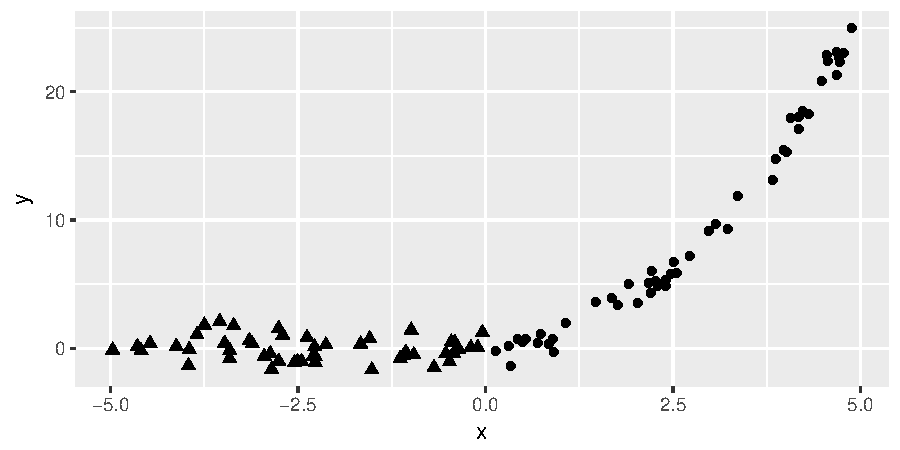
\includegraphics[width=5.5in]{nonlinear}
\end{figure}

\noindent Imagine if $\mathbb{D}$ consisted of the subset of the data pictured above where $\mathcal{X} = \braces{x : x \geq 0}$ i.e. no triangle points are part of the historical data. Consider $\mathcal{A} = $ OLS and the following model candidate sets:

\beqn
\mathcal{H}_1 &=& \braces{w_0 + w_1 x} \\
\mathcal{H}_2 &=& \braces{w_0 + w_1 x^2} \\
\eeqn

\benum

\subquestionwithpoints{3} Which model candidate set would be better for building a model $g$ using $\mathbb{D}$ whose goal is to predict in $\mathcal{X} = \braces{0, 3}$?

\begin{enumerate}[i)]
\item $\mathcal{H}_1$
\item $\mathcal{H}_2$
\item not enough information to tell
\end{enumerate}

\subquestionwithpoints{3} Which model candidate set would be better for building a model $g$ using $\mathbb{D}$ whose goal is to predict in $\mathcal{X} = \braces{-3, 3}$?

\begin{enumerate}[i)]
\item $\mathcal{H}_1$
\item $\mathcal{H}_2$
\item not enough information to tell
\end{enumerate}
\pagebreak

\subquestionwithpoints{3} Which model candidate set would be better for building a model $g$ using $\mathbb{D}$ whose goal is to predict in $\mathcal{X} = \reals$?

\begin{enumerate}[i)]
\item $\mathcal{H}_1$
\item $\mathcal{H}_2$
\item not enough information to tell
\end{enumerate}

\eenum


\problem We continue with \qu{non-linear} linear modeling. We will consider a similar-looking dataset as in the previous problem but the situation will be totally different. Below the response $y$ is plotted by predictor $x$. However there is a second dummy predictor $z$ which is pictured below as well. If $z=1$, the illustration displays a circle and if $z=0$, the illustration displays a triangle. The entire $\mathbb{D}$ is plotted below.


\begin{figure}[htp]
\centering
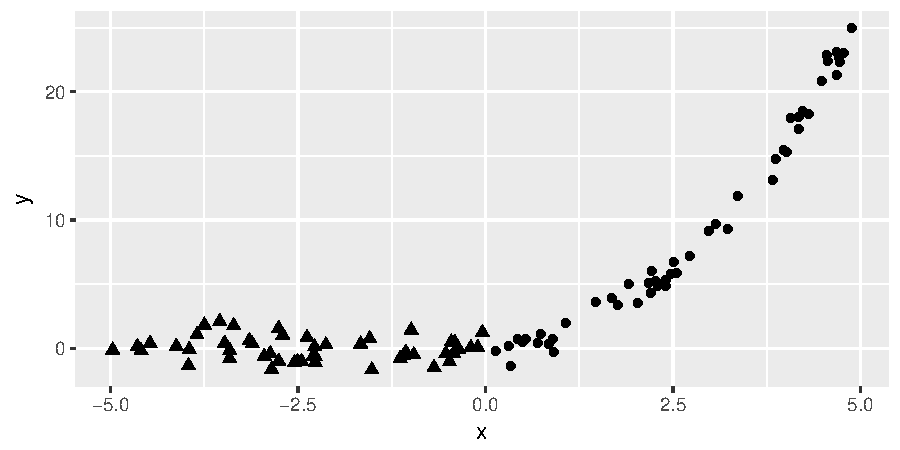
\includegraphics[width=5.3in]{nonlinear}
\end{figure}

Consider $\mathcal{A} = $ OLS and the following model candidate sets:

\beqn
\mathcal{H}_1 &=& \braces{w_0 + w_1 x} \\
\mathcal{H}_2 &=& \braces{w_0 + w_1 z} \\
\mathcal{H}_3 &=& \braces{w_0 + w_1 x^2} \\
\mathcal{H}_4 &=& \braces{w_0 + w_1 x + w_2 z + w_3 xz} \\
\eeqn

\benum

\subquestionwithpoints{3} Which model candidate set would be better for building a model $g$?

\begin{enumerate}[i)]
\item $\mathcal{H}_1$
\item $\mathcal{H}_2$
\item $\mathcal{H}_3$
\item $\mathcal{H}_4$
\item not enough information to tell
\end{enumerate}


\subquestionwithpoints{6} Regardless of your answer in (a), assume $\mathcal{H}_4$ was employed. Estimate $\b$ as best as you can.\spc{9}

\eenum

\problem This question is about general concepts of modeling including under/overfitting.

\benum

\subquestionwithpoints{6} Assume a general $\mathbb{D}$, $\mathcal{A}$ and $\mathcal{H}$ and $\mathcal{Y} \subset \reals$.  In the graph below, (1) draw the relationship between in-sample error and model complexity, (2) draw the relationship between out-of-sample error and model complexity, then (3) indicate the region of underfitting and (4) indicate the region of overfitting.  \spc{-0.5}


\begin{figure}[htp]
\centering
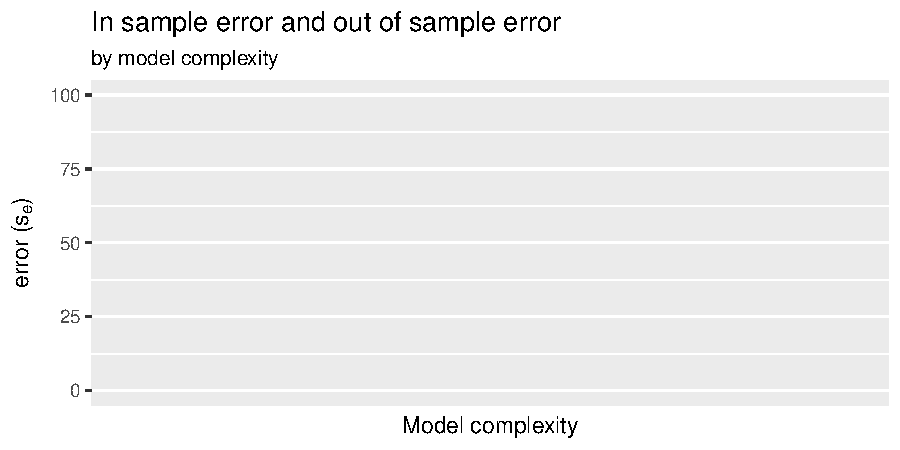
\includegraphics[width=6.5in]{complexity}
\end{figure}

\pagebreak

\subquestionwithpoints{6} Assume a general phenomenon where you're given $\mathbb{D}$ and $\mathcal{Y} \subset \reals$ and $\mathcal{A}$ and corresponds to a least squares minimization for and a simple model space $\mathcal{H}$ with 10 parameters. Assume $\epsilon$ is non-zero. Now, (1) draw the relationship between in-sample error and $n$, the number of data points in $\mathbb{D}$, (2) draw the relationship between out-of-sample error and $n$.  \spc{-0.5}


\begin{figure}[htp]
\centering
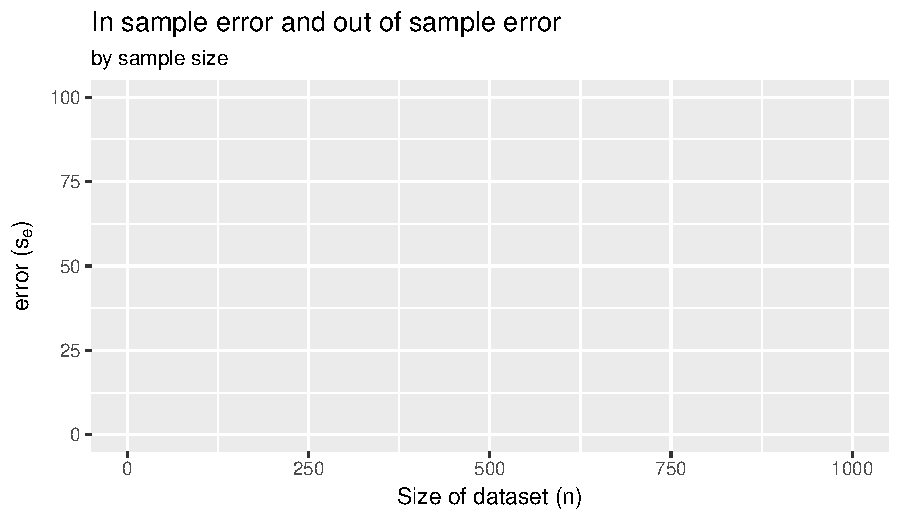
\includegraphics[width=5.35in]{n_increasing}
\end{figure}


\subquestionwithpoints{3} [Extra credit] Assume the same setup as in (b) but now the model space $\mathcal{H}$ is complex with 100 parameters. Now, (1) draw the relationship between in-sample error and $n$, the number of data points in $\mathbb{D}$, (2) draw the relationship between out-of-sample error and $n$. Make sure to indicate clearly how the relationships differ here from the relationships you drew in (b).  \spc{-0.5}


\begin{figure}[htp]
\centering
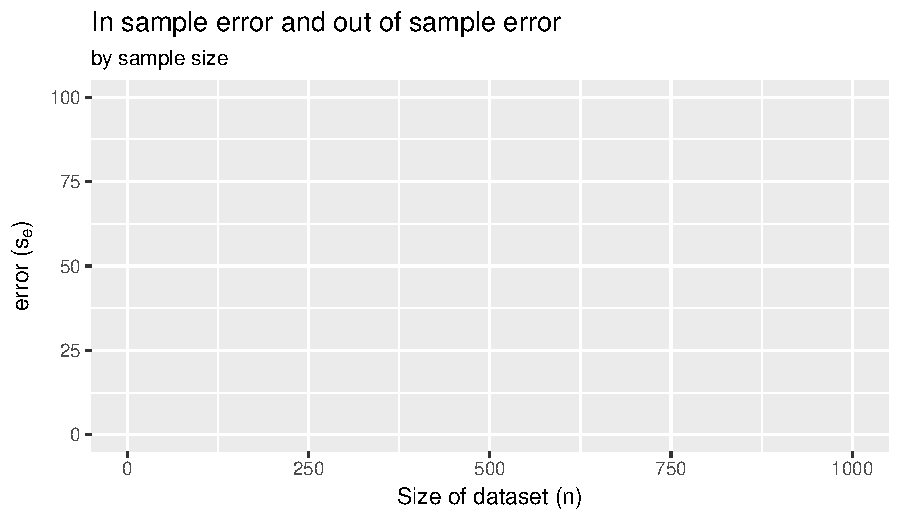
\includegraphics[width=5.35in]{n_increasing}
\end{figure}


\subquestionwithpoints{6} Consider the plot below. \spc{-0.5}


\begin{figure}[htp]
\centering
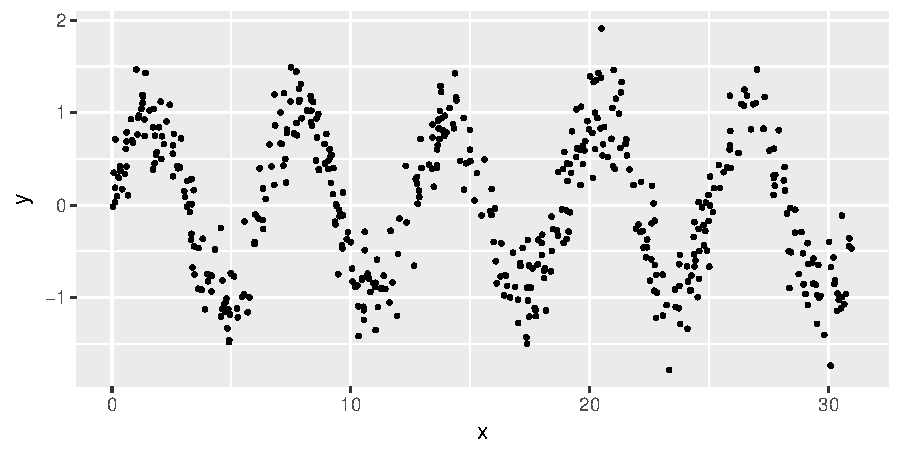
\includegraphics[width=5.5in]{sine}
\end{figure}

Which one(s) of the following statement(s) are most likely true?

\begin{enumerate}[i)]
\item the predictor $x$ and the response $y$ are correlated
\item the predictor $x$ and the response $y$ are associated
\item $s_{xy}$ will be approximately zero
\item $s_{xy}$ will be exactly zero
\item $r$ will be approximately zero
\item $r$ will be exactly zero
\item $\delta = 0$
\item $f(x) = 0$
\item the random variable $X$ (that generated the realizations of $x$ above) and the random variable $Y$ (that generated the $\iid$ realizations of $y$) are dependent
\item the random variable $X$ (that generated the realizations of $x$ above) and the random variable $Y$ (that generated the $\iid$ realizations of $y$) are independent
\item this data is only of theoretical interest and can never be found in the real world
\item a linear model with polynomial terms will take many degrees of freedom to fit well
\item a model with a intelligently selected $\mathcal{H}$ can be fit with very few degrees of freedom
\item this data can \textit{only} be fit if one uses three splits of $\mathbb{D}$ --- one for training, one for selection and one for testing
\end{enumerate}

\eenum
\pagebreak



\problem Below are some questions on the practice topics we studied. We first load the diamonds data and we remind ourselves of the response (\texttt{price}) and the 9 features:


\begin{lstlisting}
> pacman::p_load(ggplot2)
> data(diamonds)
> diamonds$cut = factor(as.character(diamonds$cut))
> diamonds$color = factor(as.character(diamonds$color))
> diamonds$clarity = factor(as.character(diamonds$clarity))
> summary(diamonds)
    carat               cut        color        clarity     
 Min.   :0.2000   Fair     : 1610   D: 6775   SI1    :13065  
 1st Qu.:0.4000   Good     : 4906   E: 9797   VS2    :12258  
 Median :0.7000   Ideal    :21551   F: 9542   SI2    : 9194  
 Mean   :0.7979   Premium  :13791   G:11292   VS1    : 8171  
 3rd Qu.:1.0400   Very Good:12082   H: 8304   VVS2   : 5066  
 Max.   :5.0100                     I: 5422   VVS1   : 3655  
                                    J: 2808   (Other): 2531  
     depth           table           price             x         
 Min.   :43.00   Min.   :43.00   Min.   :  326   Min.   : 0.000  
 1st Qu.:61.00   1st Qu.:56.00   1st Qu.:  950   1st Qu.: 4.710  
 Median :61.80   Median :57.00   Median : 2401   Median : 5.700  
 Mean   :61.75   Mean   :57.46   Mean   : 3933   Mean   : 5.731  
 3rd Qu.:62.50   3rd Qu.:59.00   3rd Qu.: 5324   3rd Qu.: 6.540  
 Max.   :79.00   Max.   :95.00   Max.   :18823   Max.   :10.740  
                                                                 
       y                z         
 Min.   : 0.000   Min.   : 0.000  
 1st Qu.: 4.720   1st Qu.: 2.910  
 Median : 5.710   Median : 3.530  
 Mean   : 5.735   Mean   : 3.539  
 3rd Qu.: 6.540   3rd Qu.: 4.040  
 Max.   :58.900   Max.   :31.800 
\end{lstlisting}
\vspace{-1cm}


\benum

\subquestionwithpoints{4} As best as you can, illustrate the output of the following code. Make sure you label axes and provide some tick marks.

\begin{lstlisting}
> ggplot(diamonds) + 
     geom_density(aes(carat))
\end{lstlisting}~\spc{6}


\subquestionwithpoints{4} We now run an anova model as follows:

\begin{lstlisting}
> anova_mod = lm(price ~ cut, diamonds)
\end{lstlisting}
\vspace{-0.8cm}

and below are the $\b$ and RMSE:

\begin{lstlisting}
> coef(anova_mod)
 (Intercept)      cutGood     cutIdeal   cutPremium cutVery Good 
   4358.7578    -429.8933    -901.2158     225.4999    -376.9979 
> summary(anova_mod)$sigma
[1] 3963.847
\end{lstlisting}
\vspace{-0.8cm}

The first six entries of the variable \texttt{cut} are:

\begin{lstlisting}
> head(diamonds$cut)
[1] Ideal     Premium   Good      Premium   Good      Very Good
Levels: Fair Good Ideal Premium Very Good
\end{lstlisting}
\vspace{-0.8cm}

Provide below the first six rows of the model matrix $\X$ for the model \texttt{price $\sim$ cut}.\spc{5}

\subquestionwithpoints{3} [Extra credit] Given the model and the results in (b), illustrate as best as you can the result of the following code. Credit will only be given to near perfect renditions.

\begin{lstlisting}
> ggplot(diamonds) + 
     geom_boxplot(aes(x = cut, y = price))
\end{lstlisting}~\spc{6}

\subquestionwithpoints{6} The first six entries of carat are 

\begin{lstlisting}
> head(diamonds$carat)
[1] 0.23 0.21 0.23 0.29 0.31 0.24
\end{lstlisting}
\vspace{-0.8cm}

Illustrate the result of the following code:

\begin{lstlisting}
> head(model.matrix(price ~ carat * cut, diamonds))
\end{lstlisting}~\spc{5}


\subquestionwithpoints{6} Consider $\mathcal{A} = $ OLS and the following models explaining diamond \texttt{price}:


\begin{enumerate}[1.]
\item a 4-degree polynomial of carat
\item all raw features
\item all features interacted with carat
\item all interactions
\end{enumerate}

Write code below to fit these four models and save them as \texttt{mod\_1}, \texttt{mod\_2}, \texttt{mod\_3}, \texttt{mod\_4}. \spc{6}

\subquestionwithpoints{4} If $R^2$ was employed to select the \qu{best} model of the four in (d), what would be the result? That is, which model would it declare the winner?\spc{0.5}

\subquestionwithpoints{5} [Extra credit] Write code below that will select the \qu{best} model of the four in (d) as measured by future predictive performance.

\eenum


\end{document}
